
% last updated in April 2002 by Antje Endemann
% Based on CVPR 07 and LNCS, with modifications by DAF, AZ and elle, 2008 and AA, 2010, and CC, 2011; TT, 2014; AAS, 2016


\documentclass[runningheads]{llncs}
%\usepackage{tikz}
\usepackage{graphicx}
\usepackage{amsmath,amssymb} % define this before the line numbering.
\usepackage{ruler}
\usepackage{color}
\usepackage[width=122mm,left=12mm,paperwidth=146mm,height=193mm,top=12mm,paperheight=217mm]{geometry}
\usepackage{url}
\usepackage{hyperref}

%\usepackage{pgfplots}

\begin{document}
% \renewcommand\thelinenumber{\color[rgb]{0.2,0.5,0.8}\normalfont\sffamily\scriptsize\arabic{linenumber}\color[rgb]{0,0,0}}
% \renewcommand\makeLineNumber {\hss\thelinenumber\ \hspace{6mm} \rlap{\hskip\textwidth\ \hspace{6.5mm}\thelinenumber}}
% \linenumbers
\pagestyle{headings}
\mainmatter
\def\ECCV16SubNumber{***}
\title{DD2424 Project - character-level text classification with different RNN architectures}

\maketitle

%The final report should include the following sections:

\begin{abstract}
% • Abstract: Where you give an overview of the task and the findings
% of your work in a nutshell.

\dots
\keywords{We would like to encourage you to list your keywords within
the abstract section}
\end{abstract}


\section{Introduction}

% • Introduction/Problem formulation: Motivate the problem you
% are trying to solve, attempt to make an intuitive description of the
% problem and also formally define the problem. (1-2 pages including
% title, authors and abstract)

We are looking at a text classification problem with short text and character-level classification. We will be using character-level classification. This means that the network processes the input one character at a time. Each character results in an output consisting of the probabilities for each letter for the next character. If we have a 58-character alphabet, the hidden state will consist of the probability of each of those 58 characters for the next letter in the sequence. So for each character, one such prediction is produced, as well as a hidden state, which is fed into the next step.

Short-text classification is hard in that there is less information to go off with little to no grammar or syntax. Some applications of short-text classification include search queries and information retrieval, mapping a product name to its associated product, the classification of titles, questions, sentences, and short messages.

The texts we are looking at are names of cities, and the classes are the names of the country the city belongs to. To begin with, we used the world-cities data set. We later abandoned it for geonames, because it has more samples. There are circa 240 categories (countries) in the data sets, but we will limit the number of categories so as not to make the categories too unevenly distributed (ie remove countries with too few cities in the data set).

The inspiration for the project is \href{https://github.com/spro/practical-pytorch/blob/master/char-rnn-classification/char-rnn-classification.ipynb}{a tutorial}
 in which a recurrent network is used to classify names as belonging to certain nationalities, using the Python framework \textit{Pytorch}. To start with, the model of that tutorial is to be replicated, then additional architectures will be implemented and compared. Questions we ask ourselves include: to what degree would a deeper network help in this problem? What sort of architectures are good in this application? Would an LSTM-layer in the recurrent network give better results? 

To measure the success of the text classification, we will look at the precision, recall and f1-score of each category in the data set. This because it gives a more nuancued evaluation than accuracy, seeing as how the data set used is heavily skewed. Furthermore, we will visualize the results with a confusion matrix.


\section{Background}

% • Background: summarize a few notable approaches/papers tackling
% the same problem. The selection should cover different possible tech-
% niques that can be (have been) used for the same task with success.
% Also, it is good to mention other recognition/synthesis tasks that use
% the same deep learning technique as yours. (1-2 pages)


\section{Approach}
% • Approach: Describe the final approach you are take for this problem.
% For instance, here you would describe the details of the network’s
% architecture. What training parameters and techniques you have used.
% The computational complexity of your model. And similar questions.
% To help explain your approach please make figures to accompany your
% text description. (1-3 pages)

\section{Experiments}

The first experiment was simply taking the model from the tutorial and running it on the first data set we had decided upon, the world-cities data set. 

The model in the tutorial looks as follows
\begin{center}
        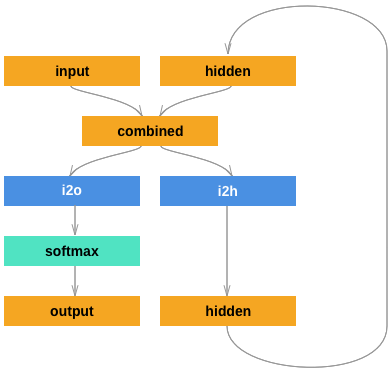
\includegraphics[width=.5\textwidth]{../plots/tutorial_model.png}
\end{center}

where i2o and i2h are simple linear layers that do a $y=Wx + b$ type calculation. Softmax is used to assign the different categories probabilities - it is a good way to represent a categorical distribution in a multi-class problem such as this one.
The criterion for loss that is used is negative log-likelihood loss.
The optimizer that is used is stochastic gradient descent. No momentum is used.
The \textit{combined} layer simply concatenates the input vector and hidden vector.

The data preprocessing was simple: the data was converted to ASCII-characters and the data was filtered to only have countries with at least 100 cities in the data set. This because the initial distribution was a bit too uneven

\begin{center}
        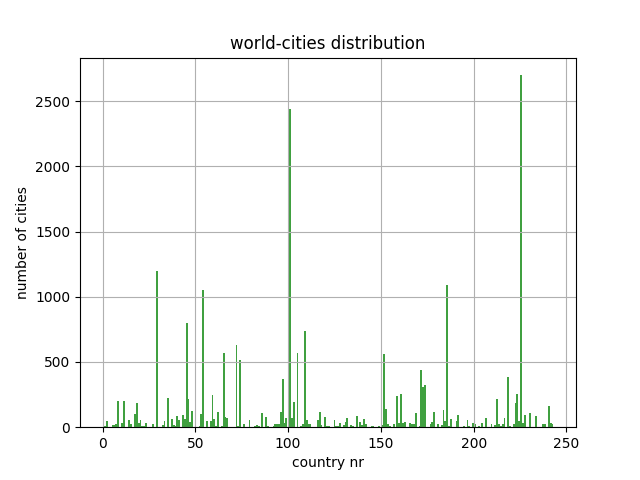
\includegraphics[width=.5\textwidth]{../plots/dist.png}
\end{center}

with many countries having very few cities, some even just 1 or 2.

What remained was 18684 data points.

The training was done in a similar way as in the tutorial, with random sampling with replacement from the data set. The final confusion matrix looked as follows

\begin{center}
        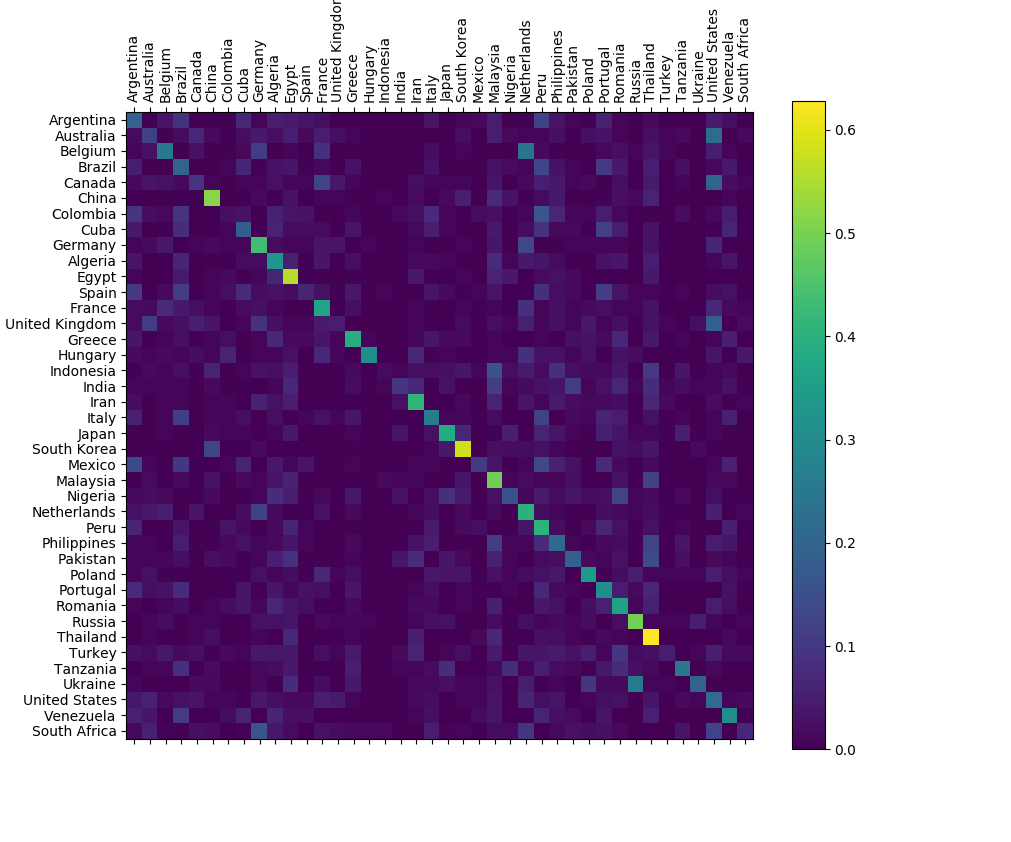
\includegraphics[width=.5\textwidth]{../plots/confusion_matrix_initial.png}
\end{center}

and the final average f1 score (averaged over all the categories) was 

While it is true that the model has a pretty good accuracy for some of the categories, it is still performing pretty unevenly for the categories. As you can see in the picture, it is pretty good at classifying countries like Thailand and Korea, but not very good at classfiying Colombia or Indonesia. We do not see a clear pattern from the class distribution (for example the US is overrepresented in the data set but is not predicted more often than other countries). This is because of how the random sampling is made - first a random category is chosen, then a sample will be taken randomly from that category. Therefore, the number of times we're exposed to samples from different categories will be more or less even.

\subsection{Introducing LSTM and GRU}

We wanted to see if an LSTM-layer could improve the performance of the network. LSTMs are units used in recurrent networks that are composed of several gates - an input gate, output gate and forget gate. The LSTM can choose to "remember" or "forget" inputs from the past. This mechanism allows them to avoid the long-term dependency problem. However, this might not matter in this particular short-text classification problem, since there should not be long-term dependencies.

LSTMs are also supposed to be good against exploding and vanishing gradients, which is a common problem in backpropagation-through-time, the most common learning algorithm for standard recurrent networks.


When we have an LSTM cell in Pytorch, it takes an input, a hidden state and a cell state and it does the following computations

\begin{gather}
	i_t = \sigma(W_{i,i} x_t + b_{i,i} + W_{h,i} h_{t-1} + b_{h,i}) \\
	f_t = \sigma(W_{i,f}x_t + b_{i,f} + W_{h,f}h_{t-1} + b_{h,f}) \\
	g_t = tanh(W_{i,g}x_t + b_{i,g} + W_{h,g}h_{t-1} + b_{h,g}) \\
	o_t = \sigma(W_{i,o}x_t + b_{i,o} + W_{h,o}h_{t-1} + b_{h,o}) \\
	c_t = f_tc_{t-1} + i_tg_t \\
	h_t = o_t tanh(c_t)
\end{gather}

where $h_t$ is the hidden state at time t, $c_t$ is the cell state at time t, $x_t$ is the input, $h_{t-1}$ is the hidden state at the previous time step and $i_t$, $f_t$, $g_t$ and $o_t$ are the input, forget, cell and output gates. \cite{torchdoc}

In other words, the LSTM cell works by applying nonlinear functions to both inputs and internal variables. 
% TODO: write more about LSTMs



\section{Results}
\section{Conclusions}

% • Experiments/Results/Conclusions: In this section, you should
% present the results you achieved with various experiments. The re-
% sults can be presented in tables, plots, etc. Explain what conclusions
% you can draw from these set of experiments? The set of experiments
% and results reported here should justify some of the design choices
% described in the previous sections. (3-6 pages)

As \cite{Alpher04} said.

% • References: It is extremely important to make sure all the content
% from other sources and the ideas that you build on are properly cited.


% Both positive and negative results should be reported. A discussion re-
% garding why certain techniques worked better than the others is necessary.
% Students are also encouraged to take initiatives in trying out new techniques,
% beyond those discussed at the lectures.
% The stated number of pages above is a guideline, one can go beyond that or
% slightly below. The whole report should be between 7-14 pages.


\bibliographystyle{splncs}
\bibliography{egbib}
\end{document}
